\capitulo{7}{Conclusiones y Líneas de trabajo futuras}

\section{Conclusiones}
Tras el desarrollo de la aplicación se han podido observar numerosos aspectos relevante sobre la calidad de cursos en línea y sobre como llegar a buenos niveles de calidad. 

En primer lugar, se debe recalcar que este proyecto tiene una base teórica muy sólida que facilita inmensamente la definición de requisitos funcionales para la aplicación. Los marcos teóricos como QRF for the MOOCs \cite{quality-reference-framework} o El estudio de modelos de calidad de elearning \cite{modelos-calidad-elearning} han ayudad a identificar claramente las reglas a seguir para hacer un desarrollo coherente basado en estudios realizados por profesionales del campo. 

Por otro lado, la elección de las herramientas y metodologías adecuadas para desarrollar esta aplicación también es relevante, dado que los productos software deben ser escalables y mantenibles en el tiempo y se necesita unos conocimientos técnicos profundos para tomar esta decisión correctamente. Además, conocimientos sobre la estructura interna del software y de su funcionamiento son necesarios, para entender cuales son las necesidades internas de la aplicación y como cubrirlas. 

ELearningQA ayuda al personal académico a ofrecer una educación en línea de calidad, para que los estudiantes puedan ser formados en las mejores condiciones y para poder aprovechar al máximo las herramientas y las ventajas que ofrece Moodle. Prueba de ello es, que en el proceso de pruebas del proyecto, los tutores involucrados localizaron en uno de sus cursos una baja participación  del alumnado a pesar de que los índices de facilidad se encuentran en valores altos entre 69\% y 88\%. Esto índica que las nuevas funcionalidades funcionan como se esperaba  y muestran de forma correcta y clara el nivel de calidad de los cuestionarios.

Como conclusión, se puede ver que el resultado final del desarrollo coincide con los objetivos planteados, esto es gracias al sistema de desarrollo con metodologías ágiles, a la utilización de las herramientas que permiten un desarrollo continuo y el apoyo de los miembros del equipo. Los objetivos principales logrados son los siguientes:
\begin{enumerate}
    \item \textbf{Realizar el mantenimiento de la aplicación:} Este proyecto no ha recibido el mantenimiento necesario para ser funcional en el tiempo, por ello ha sido necesario hacer un mantenimiento de la aplicación, realizando los cambios necesarios para que cumpla con las funciones para las que se ha desarrollado. En este mantenimiento se incluye la programación para ser compatible con las nuevas versiones de Moodle, así como para seguir siendo compatible con las anteriores. De esta forma todos los usuarios de Moodle podrán servirse de esta aplicación, aumentando así el alcance del proyecto.
    \item \textbf{Añadir nuevas reglas de cuestionarios:} Los marcos teóricos en los que se basa esta aplicación proporciona una gran variedad de requisitos para mantener la calidad de un curso en línea, esto proporciona a los desarrolladores una fuente constante de funcionalidades implementables a la aplicación. La única barrera que existe para implementar estas funcionalidades es la forma de obtener los datos, esto es una dificultad añadida, pero no hace imposible el desarrollo de nuevas funcionalidades. Así pues ha sido posible añadir cinco reglas, cuatro en la fase de realización y una en la fase de diseño, que hacen comprobaciones sobre los cuestionarios y muestran la calidad de los mismos. De este modo, los responsables del diseño e implementación de los cuestionarios tienen retroalimentación constante sobre la calidad del trabajo realizado.
    \item \textbf{Añadir nueva regla de diseño del curso:} Otra regla necesaria para conocer la calidad general del curso es la comprobación de la definición de variables, en este caso de fechas de inicio y fin y descripción del curso.
    \item \textbf{Exportación de informes a Excel:} Para poder disponer de los informes offline, se ha implementado la funcionalidad de exportar informes en Excel, de forma que los responsables académicos puedan disponer de ellos en cualquier momento.
\end{enumerate}

\section{Líneas de trabajo futuras}
Esta aplicación goza de disponer de unos requisitos funcionales bien definidos gracias a la rica base teórica de la que dispone. Además haciendo un estudio estructural de la aplicación se puede ver que existen varios aspectos mejorables.

\subsection{Nueva regla: Las preguntas de ensayo tienen una guía de calificación para profesores}
Una regla que se sitúa en la fase de diseño y que tiene como responsable al diseñador: las preguntas de ensayo tienen una guía de calificación para profesores. Esta regla corresponde al proceso D-11 del Marco de referencia de calidad para los MOOCs \cite{quality-reference-framework}. La complejidad para la implementación de esta regla se encuentra en la obtención de los datos, debido a que la API de Moodle \cite{moodle-api} no proporciona esta información. Por lo que será necesario encontrar y realizar las peticiones necesarias para obtener esta información utilizando web scraping.

\subsection{Nueva regla: Los estudiantes consultan la retroalimentación del cuestionario}
Una regla que se sitúa en la fase de evaluación y que tiene como responsable al proveedor: los estudiantes consultan la retroalimentación del cuestionario. Esta regla corresponde al proceso E-2 del Marco de referencia de calidad para los MOOCs \cite{quality-reference-framework}. Para implementar esta regla tampoco existe la posibilidad de obtener los datos vía la api de Moodle. Por ello, la dificultad de la implementación de esta regla aumenta, ya que será necesario acceder a los logs de Moodle, hacer una limpieza de estos y leer de ellos aquellos que interesan para dar los resultados. Un ejemplo de lectura de logs se puede encontrar en Ubumonitor \cite{ubu-monitor}

\subsection{Nueva regla: Los cuestionarios tienen retroalimentación definida}
Una regla que se sitúa en la fase de diseño y que tiene como responsable al diseñador: los estudiantes consultan la retroalimentación del cuestionario. Esta regla corresponde al proceso D-10 del Marco de referencia de calidad para los MOOCs \cite{quality-reference-framework}. Esta regla se puede implementar utilizando directamente la API de Moodle, por lo que es relativamente sencilla de implementar.

\subsection{Cambio estructural de la aplicación}
La importancia de la experiencia de usuario en una aplicación es casi tan importante como la funcionalidad que la aplicación proporciona. Una interfaz atractiva hará que los usuarios valoren la aplicación, y que atraiga a nuevos usuarios gracias a unas buenas primeras impresiones \cite{importancia-ux}. 

Para implementar una interfaz de usuario atractiva sería conveniente disponer de herramientas actualizadas que dispongan de librerias adecuadas para el desarrollo en frontend. Sin embargo, eLearningQA dispone de JSP para esto. Esto no significa que JSP sea una tecnología mala, mas bien desactualizada. Por ello sería mas conveniente de disponer de herramientas como Angular o React, que son Frameworks más potentes y fáciles de utilizar.

En consecuencia, sería necesario hacer una reestructuración grande para hacer este desacople de frontend y backend. Esto puede llevar a pensar que después de este cambio no tendría sentido mantener el backend, pero eso no es así, ya que este backend será el encargado de la obtención y transformación de los datos y de una posible persistencia de los mismos en el futuro.

Finalmente, con este cambio se tendría un producto software con una estructura modularizada y clara \ref{fig:aplicacion-dividida}. Aumentaría la complejidad de mantenimiento, pero también permitiría manejar la asincronía y la experiencia de usuario sería mucho mejor, existiendo la posibilidad de hacer una implementación responsive.

\begin{figure}[H]
    \centering
    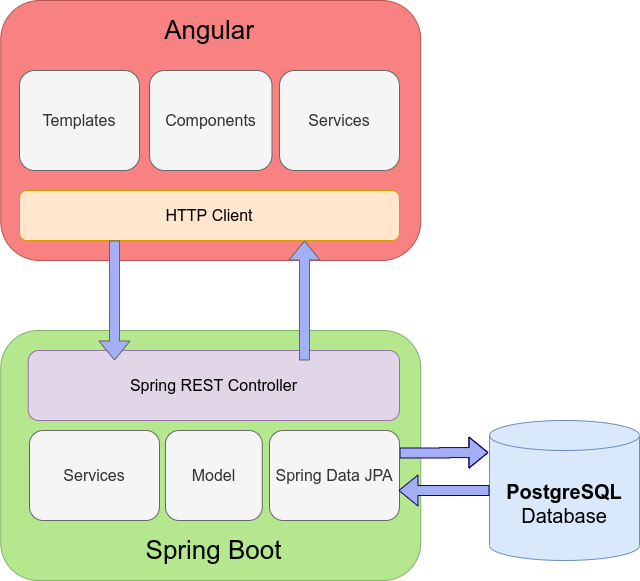
\includegraphics[width=0.80\linewidth]{img/angularMasSpring.png}
    \caption{Estructura de una apliación con Angular y Spring}
    \label{fig:aplicacion-dividida}
\end{figure}


\subsection{Mejorar la implementación del archivo de configuración}
En relación a la presentación gráfica de la aplicación y al archivo de configuración que se utiliza para el cálculo de reglas, también sería interesante que los valores del archivo de configuración, estuviese presentado en forma de formulario. De forma que cada valor estuviese ligado a cada regla que utiliza estos valores y como valores por defecto los valores fuesen los recomendados por Moodle. 

De esta forma, la configuración previa a la generación del informe sería más amigable y sencialla para el usuario.

\subsection{Internacionalización de la aplicación}
Actualmente la aplicación esta solamente en un idioma, esto limita el alcance de la aplicación a los usuarios hispanohablantes. Por ello sería interesante aumentar los idiomas en la aplicación ,con la librería i18n, como mínimo al inglés, ya que también es una de las lenguas más habladas. 

\subsection{Cálculo flexible de reglas}
Hay ocasiones en las que el usuario, no utiliza ciertas reglas o no le son útiles. Actualmente, esas reglas no deseadas por el usuario computan igualmente en la calificación global del curso. Esto es un aspecto negativo para la aplicación ya que no se adapta a las necesidades del usuario. Por ello sería interesante implementar una funcionalidad que permita desactivar ciertas reglas y que estas no computen en la puntuación global. 

También, es importante recordar que el objetivo de la aplicación es mantener un mínimo de calidad, por lo que quizás ciertas reglas nunca deberían ser desactivadas, pero eso debe someterse a estudio para tomar una decisión acertada.



